%%%%%%%%%%%%%%%%%%%%%%%%%%%%%%%%%%%%%%%%%
% University/School Laboratory Report
% This is for code review purposes only
% 
% Authors:
% Szymon Zinkowicz
%
% License:
% MIT
%
%%%%%%%%%%%%%%%%%%%%%%%%%%%%%%%%%%%%%%%%%





%----------------------------------------------------------------------------------------
%	PACKAGES AND DOCUMENT CONFIGURATIONS
%----------------------------------------------------------------------------------------



\documentclass[
	report, % Paper size, specify a4paper (A4) or letterpaper (US letter)
	11pt, % Default font size, specify 10pt, 11pt or 12pt
]{CSUniSchoolLabReport}

\usepackage[table, dvipsnames]{xcolor}
\usepackage{hyperref}
\usepackage{graphicx}
\usepackage{subcaption} % To have subfigures available
\usepackage{caption} % To have caption justification
\usepackage[export]{adjustbox}
\usepackage{lipsum} % for mock text
\usepackage{fancyhdr}
\usepackage{csvsimple} % for reading csv
\usepackage{float} % for H in figures
\usepackage{siunitx} % for SI units and rounding
\usepackage{pgfplotstable}  % For handling table imports and formatting
\usepackage{booktabs}       % For professional table formatting
\usepackage{pgffor}   % For looping constructs
\usepackage{array,multirow,makecell}
\usepackage{pdflscape}
\usepackage{forloop}  % For creating loop-like behavior
\usepackage{geometry} % For setting the margins
\newcounter{ct}
\newcommand{\addimage}[1]{%
    \begin{minipage}{0.48\textwidth}
        \centering
        \includegraphics[width=\linewidth]{#1}
    \end{minipage}%
}

\newcolumntype{R}[1]{>{\raggedleft\arraybackslash }b{#1}}
\newcolumntype{L}[1]{>{\raggedright\arraybackslash }b{#1}}
\newcolumntype{C}[1]{>{\centering\arraybackslash }b{#1}}

\sisetup{
  round-mode = places, % Rounds numbers
  round-precision = 4, % to 4 decimal places
}
\addbibresource{sample.bib} % Bibliography file (located in the same folder as the template)

\hypersetup{
	colorlinks=true,
	linktoc=all,
	linkcolor=blue,
}

\pagestyle{fancy}
\fancyhead{} % clear all header fields
\fancyfoot{} % clear all footer fields
\fancyfoot[R]{\thepage} % page number in "outer" position of footer line
\renewcommand{\headrulewidth}{2pt}
\renewcommand{\footrulewidth}{1pt}
\renewcommand{\sectionmark}[1]{\markboth{\thesection. #1}{}}
\fancyhead[L]{%
  \begin{tabular}{@{}l@{}}
  \leftmark\\
  \rightmark
  \end{tabular}%
}
\setlength{\headheight}{24pt}

%----------------------------------------------------------------------------------------
%	Functions ;>
%----------------------------------------------------------------------------------------

\newcommand{\csvtable}[3]{% #1=filename, #2=caption, #3=column headers
\begin{table}[H]
    \centering
    \rowcolors{3}{white}{lightgray}  % Start alternating colors from the 3rd row
    \csvreader[%
        tabular=|c|c|,
        table head=\hline \rowcolor{SeaGreen} #3 \\\hline,  % Apply SeaGreen to header row
        late after line=\\\hline,
        before reading={\rowcolors{3}{white}{lightgray}}  % Reinstate zebra striping after header
    ]%
    {#1}{1=\Node, 2=\Score}%
    {\Node & \Score}  % No need for \num{} unless Score data requires special formatting
    \caption{#2}
\end{table}
}


%----------------------------------------------------------------------------------------
%	REPORT INFORMATION
%----------------------------------------------------------------------------------------



\begin{document}

\title{NETWORK ANALYSIS \\
\large Assignment 3 Report \\
		Robustness analysis of a Rat Brain} % Title
\author{Szymon \textsc{Zinkowicz} \\ Matricola number: 5181814} % Author name(s)
\date{\today} % Date of the report

\maketitle % Insert the title, author, and date using the information specified above
\thispagestyle{empty}

\begin{center}
	\vspace{\fill}
	University of \textsc{Genova} \\
	\begin{tabular}{l r}
		Instructor: & Professor \textsc{Marina Ribaudo}
	\end{tabular}
\end{center}
\pagebreak



%----------------------------------------------------------------------------------------
%	Abstract
%----------------------------------------------------------------------------------------
\begin{abstract}
	\thispagestyle{empty}This study investigates the robustness of networks by comparing the effects of various node removal strategies on the structural integrity of a biological network, specifically the mouse-kasthuri-graph-v4 dataset, which simulates synaptic connections within a rat's brain. Network robustness, in this context, refers to a network's ability to maintain connectivity and function despite nodes being removed, either at random or targeted based on specific node properties. The network consists of 1,029 nodes and 1,559 edges, and comparisons were drawn with a synthetic network generated using the Barabási-Albert model.\par
	Node removal strategies implemented included random, degree, PageRank, betweenness, and closeness centrality. The resilience of the network was assessed by tracking changes in the size of the largest component and the network diameter following node removals. Findings indicate that the closeness centrality and random strategies maintained a higher level of robustness compared to other strategies, which exhibited rapid declines in the relative size of the largest component and increases in diameter during the initial phases of node removal.\par
	These observations suggest that the impact of node centrality on network robustness varies significantly across different strategies, with some strategies like closeness centrality offering more resilience, closely mimicking the effects of random failures. This highlights the potential for certain node properties to buffer against structural degradation more effectively than others.
\end{abstract}
\pagebreak

%----------------------------------------------------------------------------------------
%	Table of Contents
%----------------------------------------------------------------------------------------
\tableofcontents % Insert the table of contents
\thispagestyle{empty}
\pagebreak

\section{Introduction}

This study examines the robustness of networks by simulating random failures and targeted attacks on the \textbf{"mouse-kasthuri-graph-v4"} dataset, which represents the synaptic connections within a rat's brain. Network robustness refers to a network's ability to maintain functional connectivity despite intentional disruptions or random failures. This investigation is crucial for understanding how biological networks withstand environmental stresses and targeted disruptions, which can inform broader applications in biological and technological systems. The methods applied in this study are designed to systematically dismantle the network through various node removal strategies and observe the resulting changes in network structure and functionality.

\subsection{Methods}

The \textbf{"mouse-kasthuri-graph-v4"} dataset, consisting of 1,029 nodes and 1,559 edges, serves as the primary model for this exploration. The following node removal strategies and analyses were employed to assess the impact of these disruptions on the network's integrity:

\begin{itemize}
	\item \textbf{Node Removal Strategies:} Implementation of node failures through:
\begin{itemize}
	\item \textbf{Random Removal:} Nodes are removed at random, simulating unexpected failures.
	\item \textbf{Degree-Based Removal:} Nodes with the highest degree are targeted, representing attacks aimed at disrupting the most connected nodes.
	\item \textbf{PageRank-Based Removal:} Removal based on the highest PageRank scores to simulate attacks on the most influential nodes within the network.
	\item \textbf{Betweenness Centrality Removal:} Targeting nodes with high betweenness centrality to affect nodes that act as critical bridges within the network.
	\item \textbf{Closeness Centrality Removal:} Nodes with high closeness centrality are removed, targeting those that can spread effects most quickly across the network.
\end{itemize}
	\item \textbf{Impact Analysis:}
\begin{itemize}
	\item \textbf{Size of the Largest Component:} Monitoring changes in the size of the largest connected component as nodes are removed, which helps gauge the network's ability to remain coherent under stress.
	\item \textbf{Diameter of the Largest Component:} Observing changes in the diameter of the largest connected component of the network, which reflects the maximum distance between any two nodes in the largest subset of the network that remains connected. This metric is crucial for understanding how the structural integrity of the network changes in response to node removals.
	\begin{itemize}
		\item Scale-free networks are more resilient against random attacks compared to centrality-based attacks, mainly because random attacks are less likely to immediately target the critical hubs. Therefore, their diameter may not increase significantly until many nodes are removed.
	\end{itemize} 
	\end{itemize}
\end{itemize}

\subsection{Theoretical Foundations}
Network resilience is often evaluated through two principal dynamics: the size of the largest connected component (LCC) and changes in the LCC's diameter following node removal. The robustness of a network against random failures or targeted attacks can generally be predicted based on:
\begin{itemize}
    \item \textbf{Degree Distribution:} Networks with a heterogeneous degree distribution, such as scale-free networks, are typically more robust against random failures but vulnerable to attacks targeting high-degree nodes.
    \item \textbf{Clustering Coefficient and Path Length:} High clustering coefficients and short average path lengths tend to enhance a network`s resilience by providing multiple pathways for maintaining connectivity.
    \item \textbf{Centrality Measures:} Nodes identified with high centrality measures (degree, betweenness, closeness, and PageRank) play significant roles in network connectivity. Removing these nodes can disproportionately disrupt network structure and function.
\end{itemize}
\subsection{Theoretical Foundations: Molloy-Reed Criterion}
Following Molloy-Reed Criterion, after removal of a fraction of nodes greater than critical threshold a random graph is expected to contain a giant component, crucial for ensuring network functionality after node removals. The critical threshold, $f_c$, is defined as the fraction of nodes that must be removed to disintegrate the giant component. For a network with a given degree distribution, $P(k)$, the critical threshold can be calculated as:
\begin{equation}
    f_c = 1 - \frac{1}{
		\frac{\langle k^2 \rangle}
			{\langle k \rangle} - 1}
\end{equation}
If the network is random then $\langle k^2 \rangle = \langle k \rangle$ and $f_c = 1 - \frac{1}{\langle k \rangle}$, which is the critical threshold for random networks.\par
This insight is particularly relevant for networks like those generated by the Barabási-Albert model, which are scale-free and characterized by a power-law degree distribution. Such networks might remain robust under random failures due to the persistence of the giant component largely supported by a few high-degree nodes. However, they are particularly vulnerable to attacks targeted at these hubs, as the removal of even a small fraction of these nodes can lead to a rapid disintegration of the giant component.\par


\subsection{Dataset Description}
The "mouse-kasthuri-graph-v4" dataset, derived from the somatosensory cortex of a mouse brain, serves as the basis for our network analysis. This dataset is part of the broader efforts by Neurodata's Kasthuri project to provide high-resolution electron microscopy data of neural connectivity, facilitating the exploration of complex biological networks.\par


\subsubsection{Source and Collection}

Sourced from the Kasthuri lab and available through networkrepository.com, this dataset allows us to map a real biological network onto a computational model to study the spread of infectious diseases.

\subsubsection{Characteristics}
		
The dataset features a network graph with the following properties:
\begin{itemize}
	\item \textbf{Number of Nodes:} 1029, representing various cellular components within the brain.
	\item \textbf{Number of Edges:} 1559, indicative of the synaptic connections between these components.
	\item \textbf{Average Degree:} Approximately \num{3.0301263362487854}, reflecting the average number of connections per node.
	\item \textbf{Network Type:} Unweighted and undirected, suitable for fundamental network analysis.
\end{itemize}
\vspace{10pt}

This detailed structural and functional representation provides a unique platform for studying the dynamics of disease spread and assessing the impact of network topology on epidemiological outcomes. In order to prune network from nodes that are not connected, the largest subgraph with a minimum degree of 2 was extracted, resulting in a core network with\textbf{477 nodes}. This core network represents the most densely connected regions of the original dataset, providing a focused model for studying network robustness and resilience.

\subsection{Critical thresholds}

\csvtable{../out/critical_thresholds.csv}{Critical Thresholds of Graphs}{Graph & Critical Threshold}

\section{Analysis and Interpretation}

In this section, we delve into the robustness of the rat brain network and a comparative synthetic random network under various attack strategies. The focus of the analysis is on how these networks react to targeted and random node removals, specifically examining the resilience of the networks as measured by the size of the largest connected component (LCC) and the changes in the diameter of this component. By applying five distinct node removal methods—random, degree, PageRank, betweenness, and closeness centrality—we assess which strategies lead to the most significant degradation in network structure and functionality.\par

The forthcoming plots provide a visual representation of these effects, illustrating two critical metrics:
\begin{itemize}
	\item \textbf{Robustness (Size of LCC):} This metric captures the network's ability to maintain connectivity and functionality despite node removals, reflecting the network's structural integrity.
	\item  \textbf{Diameter Changes of LCC:} This metric tracks the maximum distance between any two nodes within the largest connected component, offering insights into the potential increase in operational inefficiencies as the network structure is compromised.
\end{itemize}



The analysis will proceed with a detailed examination of the resulting plots, followed by a discussion of the implications of these findings for network design and protection strategies.

The following subsection will display and discuss four critical plots that encapsulate the comparative dynamics between the two networks under the specified attack methods. These visual representations are pivotal for understanding the differential impact of strategic node removals on network connectivity and functionality.
\pagebreak
\subsection{Robustness and Diameter Changes Under Various Attack Strategies}
\begin{figure}[H]
    \centering
	\captionsetup{justification=centering}
    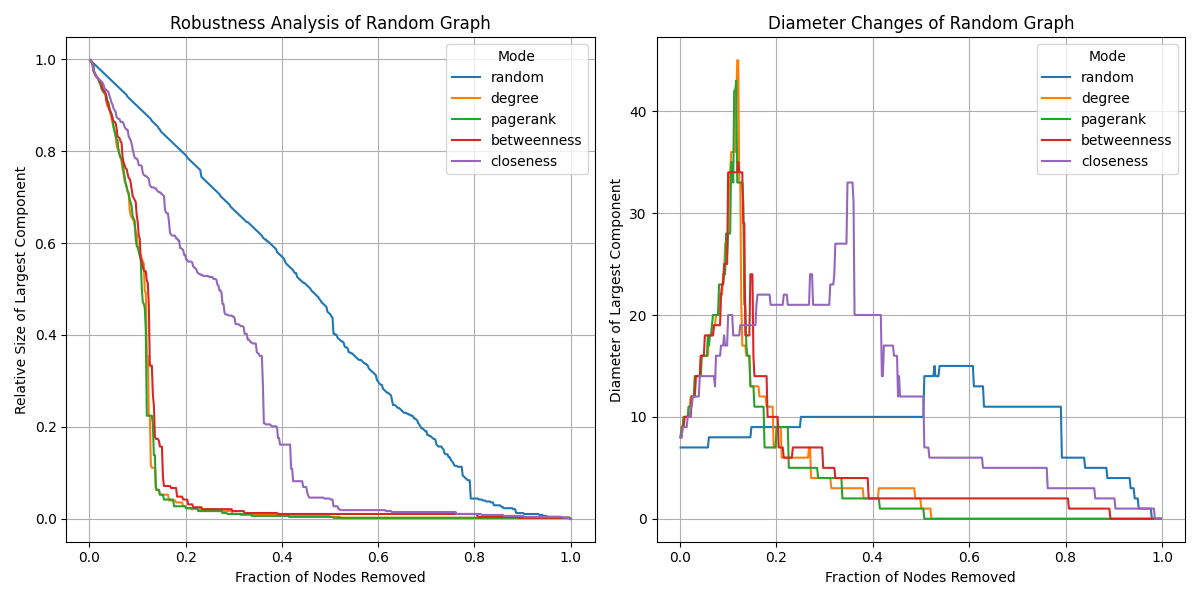
\includegraphics[width=\linewidth]{../plots/robustness-diameter-analysis-random-graph.png}
    \caption{Changes in the size of the LCC for the rat brain network under random attacks.}
    \label{fig:rat_random_lcc}
\end{figure}

\begin{figure}[H]
    \centering
	\captionsetup{justification=centering}
	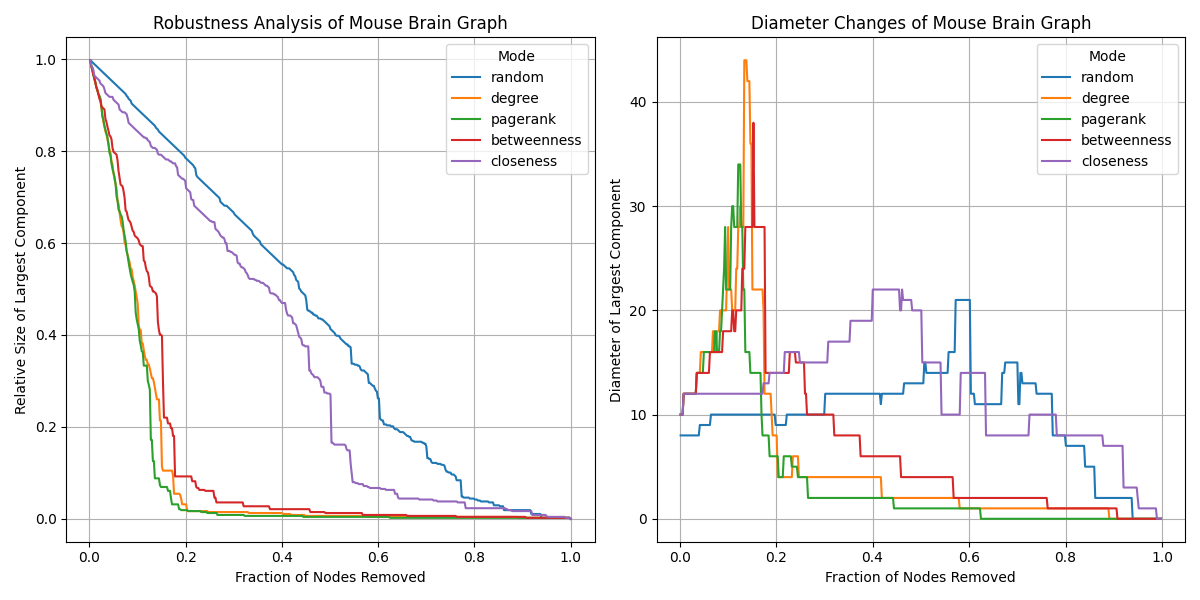
\includegraphics[width=\textwidth]{../plots/robustness-diameter-analysis-mouse-brain-graph.png}
    \caption{Changes in the diameter of the LCC for the rat brain network under random attacks.}
    \label{fig:rat_random_diameter}
\end{figure}

\clearpage
\subsection{Discussion of Findings}

The analysis of network robustness through the visualization of changes in the LCC size and diameter under various node removal strategies reveals distinct patterns of resilience and vulnerability. The plots (Figures \ref{fig:rat_random_lcc} and \ref{fig:rat_random_diameter}) illustrate how the structural integrity of networks is impacted differently by each strategy.
\subsection{Ranking of Strategies}
Each strategy is ranked from 1 to 5, with 1 being the most effective at maintaining robustness (i.e., preserving the size of the Largest Connected Component (LCC)) and minimizing diameter changes under attack. Higher ranks indicate greater vulnerability and more significant diameter increase, suggesting less effectiveness in preserving the network structure during node removal.
\begin{table}[H]
	\centering
	\captionsetup{justification=centering}
	\rowcolors{2}{white}{lightgray}
	\begin{tabular}{|c|c|c|}
		\hline
		\rowcolor{SeaGreen} \textbf{Strategy} & \textbf{Robustness Rank (LCC)} & \textbf{Diameter Change Rank} \\ \hline
		Random            & 1                              & 1                             \\ \hline
		Degree            & 5                              & 5                             \\ \hline
		PageRank          & 4                              & 4                             \\ \hline
		Betweenness       & 3                              & 3                             \\ \hline
		Closeness         & 2                              & 2                             \\ \hline
	\end{tabular}
	\caption{Ranking of Node Removal Strategies Based on Their Impact on Network Robustness and Diameter Changes.}
\end{table}

\paragraph{Impact of Random Failures}
In random failures, both networks displayed a gradual decline in the size of the LCC, indicating a level of initial robustness to sporadic node losses. However, the rat brain network showed a slightly more resilient structure compared to the synthetic network especially with defense against closeness strategy attack, possibly due to its unique biological configuration.

\paragraph{Targeted Attacks}
Contrastingly, targeted attacks, especially those based on pagerank, degree and betweenness centrality, led to a more precipitous drop in LCC size, underscoring the critical role played by highly connected and centrally located nodes. Notably, the diameter of the LCC spiked dramatically as key nodes were removed, highlighting increased path lengths among remaining nodes.

\subsection{Implications of Results}

These findings have profound implications for the design and analysis of resilient network structures. The vulnerability of networks to targeted attacks suggests that protective measures could focus on enhancing the redundancy of connections among high-centrality nodes.

\subsection{Integration of Theory and Practice}

The theoretical framework posited that networks with heterogeneous degree distributions would exhibit particular vulnerability to degree-based removals, a prediction that was borne out in the empirical data. This integration of theory and observed outcomes enriches our understanding of network dynamics and robustness, providing valuable insights for both theoretical exploration and practical application in network design and defense strategies.

\clearpage
\subsection{Conclusions}
This study provided a comprehensive analysis of network robustness by simulating random failures and targeted attacks on both a biological network modeled after the rat brain and a synthetic Barabási-Albert scale-free network. The application of the Molloy-Reed Criterion revealed critical thresholds beyond which the networks failed to maintain their giant component, significantly impacting their functionality and connectivity.\par
\begin{itemize}
    \item The critical threshold calculations indicated that the rat brain network exhibits a higher resilience against random failures compared to the synthetic network, maintaining its giant component until a higher fraction of nodes were removed. This underscores the network's robust biological architecture that might be optimized for resilience.
    \item Conversely, the Barabási-Albert model, while generally robust under random node removals, showed marked vulnerability when high-degree nodes were targeted. This finding aligns with the theoretical prediction that scale-free networks are susceptible to attacks focused on their most connected nodes.
    \item The empirical observations from the simulations supported these theoretical insights, with the network diameter and the size of the largest connected component responding as predicted by the critical thresholds.
\end{itemize}

\subsection{Recommendations for Future Research}
Further research should explore the robustness of various network types under more dynamic conditions, including adaptive networks where links can evolve in response to failures. Additionally, the application of these findings to real-world infrastructures, such as power grids and communication networks, could provide practical benefits in enhancing their resilience against both random and deliberate disruptions.

\subsection{Limitations and Future Work}
While this study provides valuable insights, it is limited by the static nature of the network models used and the focus on only two types of networks-biological and random one. Future work should consider a broader array of network models, including directed and weighted networks, to fully understand the nuances of network robustness. Additionally, incorporating feedback mechanisms where networks can reorganize in response to attacks could offer deeper insights into the resilience capabilities inherent to different network architectures.

\end{document}